\begin{frame}[t]{Implementation}

  \hspace*{.6in}
  \begin{minipage}{3.5in}
  \begin{center}

	\textbf{Pointer based file system implementation}
	\begin{itemize}
	\renewcommand{\labelitemi}{$\bullet$}
		\item Create or modify existing system
		\item Hash entire file to show matches
		\item Reduce duplicates to one file, replace removed with pointer
		\item Automatically overwrite pointers if file is modified
		\item Track all non-system files in simple database
	\end{itemize}	  
	  
	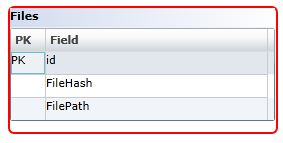
\includegraphics[scale=.7]{schema.JPG}

  \end{center}
  \end{minipage}

\end{frame}